
\documentclass[border=10pt, 12pt]{standalone}
\usepackage[svgnames]{xcolor}
\usepackage{amsmath}
\usepackage{pgfplots}
\pgfplotsset{compat=newest}
\usepackage[sfdefault]{FiraSans}
\usepackage{FiraMono}
\renewcommand*\familydefault{\sfdefault}
\begin{document}
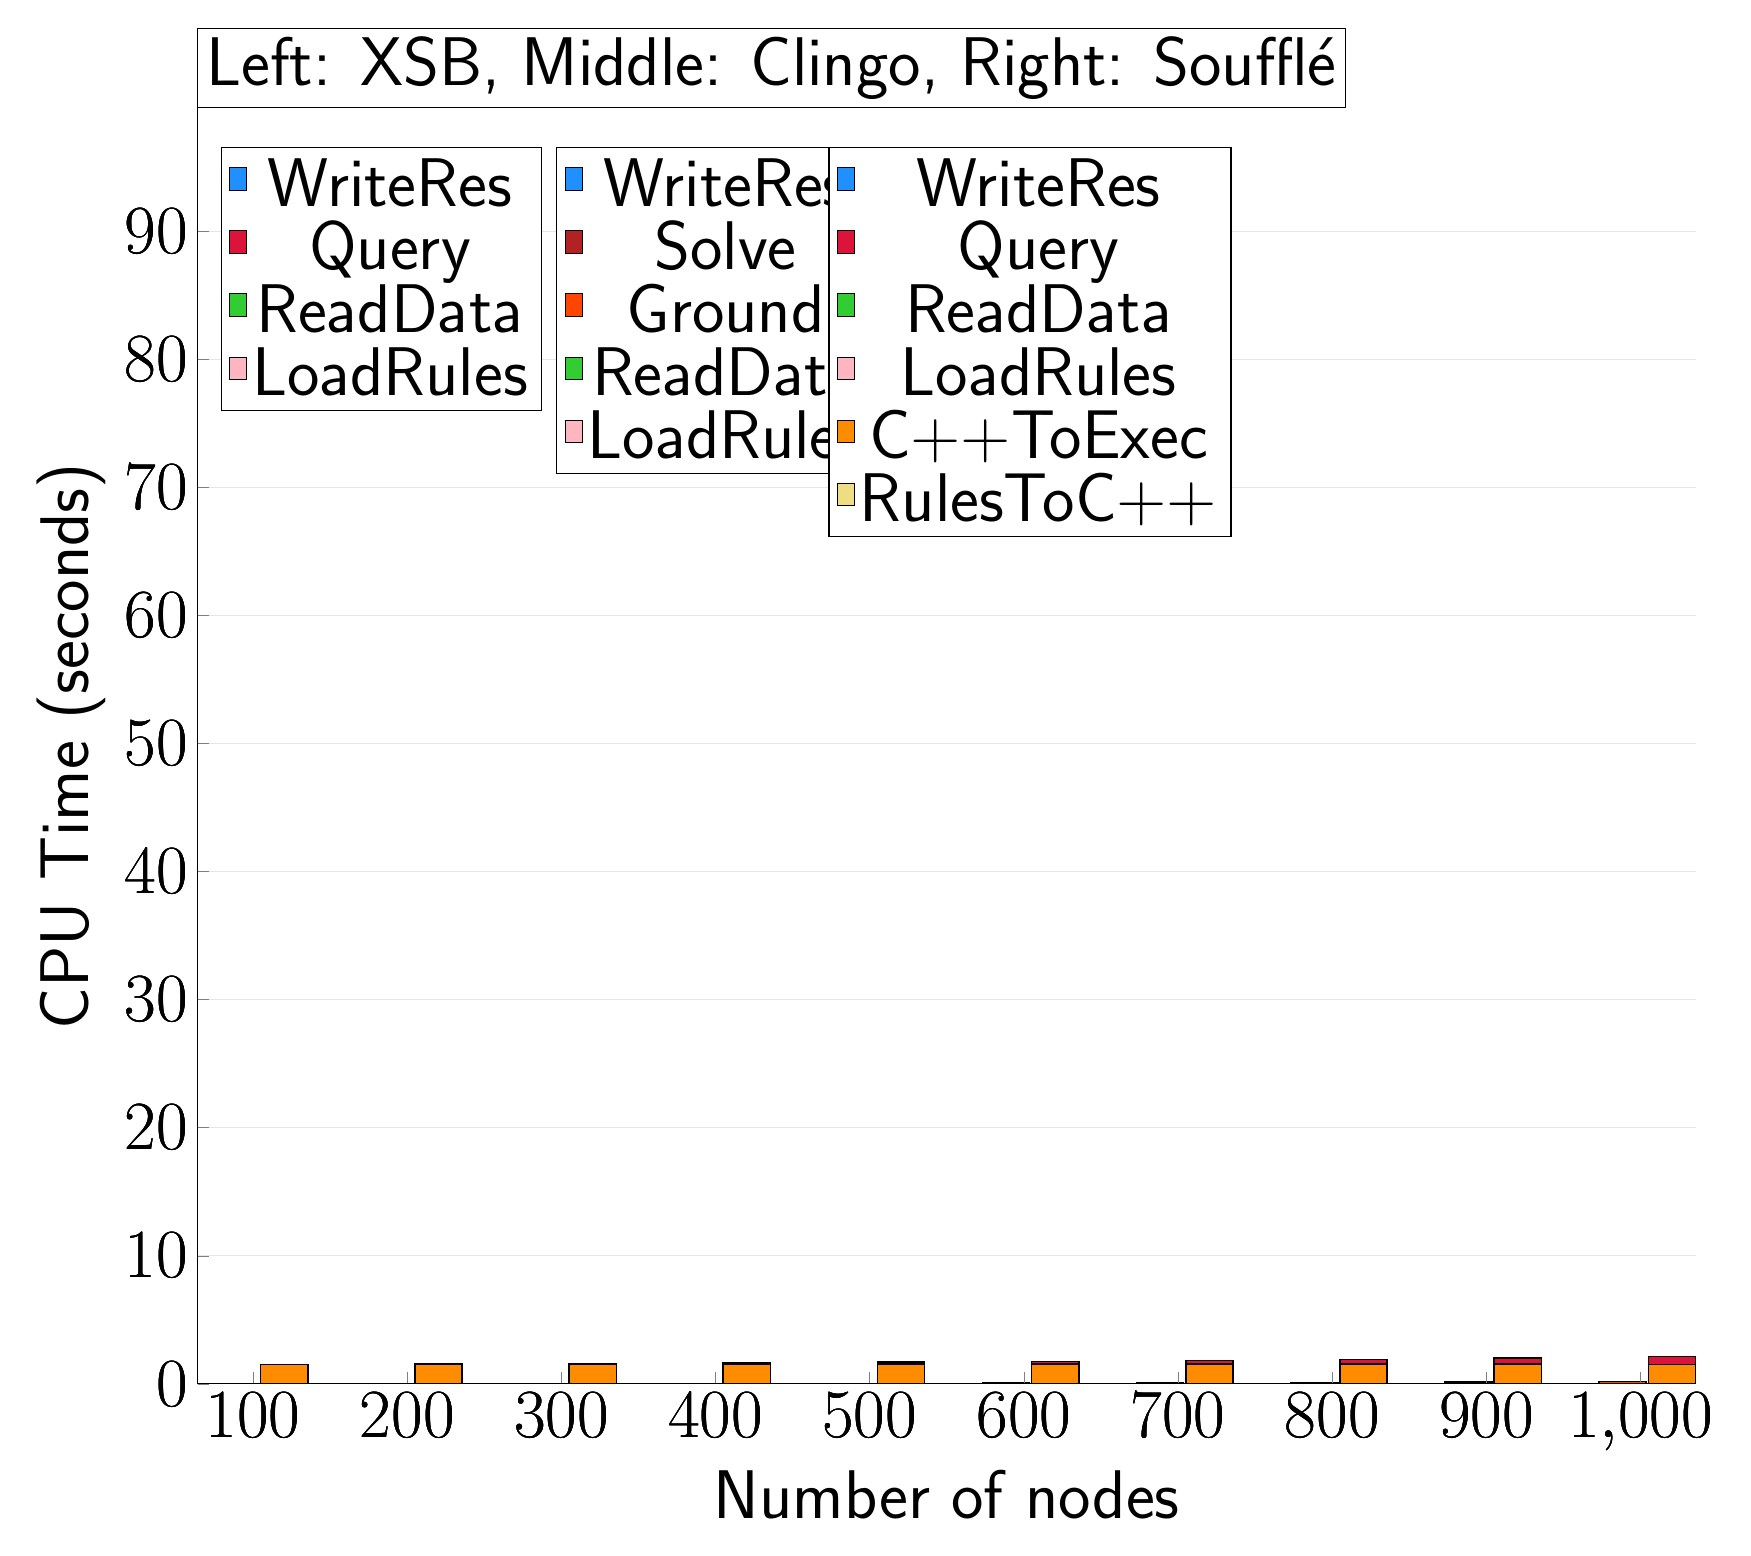
\begin{tikzpicture}
                        \begin{axis}[bar shift=-24.3pt, 
   ybar stacked,
   width=1.7\textwidth,
   bar width=0.6cm,
   ymajorgrids, tick align=inside,
   major grid style={draw=gray!20},
   xtick=data,
   ymin=0, ymax=99.5987,
   axis x line*=bottom,
   axis y line*=left,
   enlarge x limits=0.04,
   legend style={
       at={(0.23, 0.97)},
       anchor=north east,
       legend columns=1,
       font=\Huge,
   },
   ylabel={CPU Time (seconds)},
   xlabel={Number of nodes},
   label style={font=\Huge},
   tick label style={font=\Huge},
]
\addlegendimage{fill=DodgerBlue, draw=black, line width=0.2pt}
\addlegendentry{WriteRes}
\addlegendimage{fill=Crimson, draw=black, line width=0.2pt}
\addlegendentry{Query}
\addlegendimage{fill=LimeGreen, draw=black, line width=0.2pt}
\addlegendentry{ReadData}
\addlegendimage{fill=LightPink, draw=black, line width=0.2pt}
\addlegendentry{LoadRules}
\addplot +[fill=LightPink, draw=black, line width=0.55pt] coordinates {
(100, 0.0005703999999999999)
(200, 0.0005533999999999997)
(300, 0.0005608000000000004)
(400, 0.0005563999999999998)
(500, 0.0005565999999999997)
(600, 0.00056)
(700, 0.0005511999999999996)
(800, 0.0005504)
(900, 0.0005504000000000004)
(1000, 0.0005484000000000006)
};
\addplot +[fill=LimeGreen, draw=black, line width=0.55pt] coordinates {
(100, 0.0002027999999999996)
(200, 0.000276)
(300, 0.0003527999999999994)
(400, 0.00043400000000000003)
(500, 0.0005110000000000005)
(600, 0.0005945999999999996)
(700, 0.0006744)
(800, 0.0007474000000000003)
(900, 0.0008322000000000003)
(1000, 0.0009235999999999995)
};
\addplot +[fill=Crimson, draw=black, line width=0.55pt] coordinates {
(100, 1.6000000000000396e-05)
(200, 2.520000000000024e-05)
(300, 3.100000000000048e-05)
(400, 4.120000000000028e-05)
(500, 5.140000000000006e-05)
(600, 5.980000000000012e-05)
(700, 6.860000000000027e-05)
(800, 7.619999999999953e-05)
(900, 8.659999999999953e-05)
(1000, 9.260000000000033e-05)
};
\addplot +[fill=DodgerBlue, draw=black, line width=0.55pt] coordinates {
(100, 9.17999999999992e-05)
(200, 0.00012219999999999977)
(300, 0.00015739999999999933)
(400, 0.00018519999999999973)
(500, 0.00021599999999999996)
(600, 0.00024660000000000014)
(700, 0.00028140000000000033)
(800, 0.0003086000000000003)
(900, 0.00033940000000000044)
(1000, 0.0003734000000000001)
};
\end{axis}

\begin{axis}[bar shift=-6.5pt, 
   ybar stacked,
   width=1.7\textwidth,
   bar width=0.6cm,
   ymajorgrids, tick align=inside,
   major grid style={draw=none},
   xtick=data,
   ymin=0, ymax=99.5987,
   axis x line*=none,
   axis y line*=none,
   enlarge x limits=0.04,
   legend style={
       at={(0.454, 0.97)},
       anchor=north east,
       legend columns=1,
       font=\Huge,
   },
   label style={font=\Huge},
   tick label style={font=\Huge},
]
\addlegendimage{fill=DodgerBlue, draw=black, line width=0.2pt}
\addlegendentry{WriteRes}
\addlegendimage{fill=FireBrick, draw=black, line width=0.2pt}
\addlegendentry{Solve}
\addlegendimage{fill=OrangeRed, draw=black, line width=0.2pt}
\addlegendentry{Ground}
\addlegendimage{fill=LimeGreen, draw=black, line width=0.2pt}
\addlegendentry{ReadData}
\addlegendimage{fill=LightPink, draw=black, line width=0.2pt}
\addlegendentry{LoadRules}
\addplot +[fill=LightPink, draw=black, line width=0.55pt] coordinates {
(100, 0.0020000000000000018)
(200, 0.0)
(300, 0.0)
(400, 0.0)
(500, 0.0)
(600, 0.0)
(700, 0.0)
(800, 0.0)
(900, 0.0)
(1000, 0.0)
};
\addplot +[fill=LimeGreen, draw=black, line width=0.55pt] coordinates {
(100, 0.0)
(200, 0.0)
(300, 0.0)
(400, 0.0)
(500, 0.0)
(600, 0.0)
(700, 0.0)
(800, 0.0)
(900, 0.0)
(1000, 0.0020000000000000018)
};
\addplot +[fill=OrangeRed, draw=black, line width=0.55pt] coordinates {
(100, 0.0)
(200, 0.008000000000000007)
(300, 0.010000000000000009)
(400, 0.02200000000000002)
(500, 0.040000000000000036)
(600, 0.06)
(700, 0.09000000000000002)
(800, 0.11200000000000003)
(900, 0.14600000000000002)
(1000, 0.188)
};
\addplot +[fill=FireBrick, draw=black, line width=0.55pt] coordinates {
(100, 0.0)
(200, 0.0)
(300, 0.0)
(400, 0.0040000000000000036)
(500, 0.0)
(600, 0.0040000000000000036)
(700, 0.0)
(800, 0.003999999999999981)
(900, 0.0040000000000000036)
(1000, 0.0040000000000000036)
};
\addplot +[fill=DodgerBlue, draw=black, line width=0.55pt] coordinates {
(100, 0.0)
(200, 0.0)
(300, 0.0)
(400, 0.0)
(500, 0.0)
(600, -2.7755575615628915e-18)
(700, 0.0)
(800, -0.003999999999999981)
(900, -0.0040000000000000036)
(1000, -0.0040000000000000036)
};
\end{axis}

\begin{axis}[bar shift=11.3pt, 
   ybar stacked,
   width=1.7\textwidth,
   bar width=0.6cm,
   ymajorgrids, tick align=inside,
   major grid style={draw=none},
   xtick=data,
   ymin=0, ymax=99.5987,
   axis x line*=none,
   axis y line*=none,
   enlarge x limits=0.04,
   legend style={
       at={(0.69, 0.97)},
       anchor=north east,
       legend columns=1,
       font=\Huge,
   },
   label style={font=\Huge},
   tick label style={font=\Huge},
]
\addlegendimage{fill=DodgerBlue, draw=black, line width=0.2pt}
\addlegendentry{WriteRes}
\addlegendimage{fill=Crimson, draw=black, line width=0.2pt}
\addlegendentry{Query}
\addlegendimage{fill=LimeGreen, draw=black, line width=0.2pt}
\addlegendentry{ReadData}
\addlegendimage{fill=LightPink, draw=black, line width=0.2pt}
\addlegendentry{LoadRules}
\addlegendimage{fill=DarkOrange, draw=black, line width=0.2pt}
\addlegendentry{C++ToExec}
\addlegendimage{fill=LightGoldenrod, draw=black, line width=0.2pt}
\addlegendentry{RulesToC++}
\addplot +[fill=LightGoldenrod, draw=black, line width=0.55pt] coordinates {
(100, 0.0)
(200, 0.0020000000000000005)
(300, 0.008000000000000002)
(400, 0.008000000000000002)
(500, 0.010000000000000002)
(600, 0.010000000000000002)
(700, 0.010000000000000002)
(800, 0.006000000000000001)
(900, 0.008000000000000002)
(1000, 0.008000000000000002)
};
\addplot +[fill=DarkOrange, draw=black, line width=0.55pt] coordinates {
(100, 1.514)
(200, 1.53)
(300, 1.526)
(400, 1.534)
(500, 1.52)
(600, 1.528)
(700, 1.5260000000000002)
(800, 1.528)
(900, 1.53)
(1000, 1.508)
};
\addplot +[fill=LightPink, draw=black, line width=0.55pt] coordinates {
(100, 0.0001414)
(200, 0.0001482)
(300, 0.0001588)
(400, 0.000149)
(500, 0.0001304)
(600, 0.0001504)
(700, 0.0001472)
(800, 0.0001596)
(900, 0.00014419999999999998)
(1000, 0.00015120000000000002)
};
\addplot +[fill=LimeGreen, draw=black, line width=0.55pt] coordinates {
(100, 0.0008642000000000001)
(200, 0.0012182)
(300, 0.0016382)
(400, 0.0020128000000000004)
(500, 0.0021688)
(600, 0.0027218000000000003)
(700, 0.0031551999999999995)
(800, 0.0034102)
(900, 0.0034844)
(1000, 0.0037635999999999998)
};
\addplot +[fill=Crimson, draw=black, line width=0.55pt] coordinates {
(100, 0.009730800000000001)
(200, 0.0354004)
(300, 0.067496)
(400, 0.10575540000000001)
(500, 0.1536676)
(600, 0.21744819999999998)
(700, 0.29225819999999997)
(800, 0.3795674)
(900, 0.4783284)
(1000, 0.5979715999999999)
};
\addplot +[fill=DodgerBlue, draw=black, line width=0.55pt] coordinates {
(100, 0.00027100000000000003)
(200, 0.00028460000000000003)
(300, 0.0002474)
(400, 0.0002582)
(500, 0.00026039999999999993)
(600, 0.0002634)
(700, 0.00028599999999999996)
(800, 0.0003316)
(900, 0.0003118)
(1000, 0.00033099999999999997)
};
\end{axis}


\node[anchor=south, draw, fill=white] at (rel axis cs:0.42,1) {\Huge Left: XSB, Middle: Clingo, Right: Soufflé};
\end{tikzpicture}
\end{document}
                    